\documentclass[aspectratio=169, 11pt, t, xcolor={table}]{beamer}
% Slides of the English course "Computer Architecture" (same theme as the
% ENSB decks: light background, teal + orange). Compile from en/slides/.
\usepackage{amsmath, amssymb}
\usepackage{booktabs, colortbl, tabularx, array}
\usepackage{tikz}
\usepackage[skins]{tcolorbox}
\usepackage{fontawesome5}
\usepackage{listings}
\usepackage{fontspec}
\usetikzlibrary{positioning, calc, arrows.meta, shapes.geometric, decorations.pathreplacing}

\setsansfont{texgyreheros}[Extension=.otf, UprightFont=*-regular, BoldFont=*-bold,
    ItalicFont=*-italic, BoldItalicFont=*-bolditalic]
\newfontfamily\codefont[Scale=0.95, BoldFont=lmmonolt10-bold.otf,
    ItalicFont=lmmono10-italic.otf]{lmmono10-regular.otf}

\definecolor{brandTeal}{HTML}{5CC8E6}
\definecolor{brandOrange}{HTML}{FFA27F}
\definecolor{brandLight}{HTML}{F8F9FA}
\definecolor{brandDark}{HTML}{263238}
\definecolor{brandMuted}{HTML}{6C757D}
\definecolor{brandGreen}{HTML}{7BC47F}
\definecolor{brandPurple}{HTML}{B39DDB}
\colorlet{tealDeep}{brandTeal!60!black}
\colorlet{orangeDeep}{brandOrange!70!black}
\definecolor{codeGrey}{HTML}{F1F3F5}

\setbeamercolor{background canvas}{bg=brandLight}
\setbeamercolor{normal text}{fg=brandDark}
\setbeamercolor{structure}{fg=brandTeal}
\setbeamertemplate{navigation symbols}{}
\setbeamertemplate{frametitle}{%
    \vspace{0.35cm}
    \noindent{\bfseries\Large\color{brandDark}\insertframetitle}\par
    \vskip-2pt\noindent{\color{brandTeal}\rule{\textwidth}{1.5pt}}\vspace{0.05cm}}
\setbeamertemplate{footline}{%
    \hbox to \paperwidth{\hspace{0.6cm}{\color{brandMuted}\scriptsize\insertshorttitle}\hfill
        {\color{brandMuted}\scriptsize\insertframenumber\,/\,\inserttotalframenumber}\hspace{0.6cm}}%
    \vspace{0.25cm}}
\setbeamertemplate{itemize item}{\color{brandTeal}\small\faChevronRight}
\setbeamertemplate{itemize subitem}{\color{brandMuted}\small\faAngleRight}
\setbeamertemplate{enumerate item}{\color{tealDeep}\bfseries\insertenumlabel.}
% list lines are 1.4 cm apart (baseline to baseline)
\newlength{\lineGap}\setlength{\lineGap}{1.4cm}
\let\origlist\list
\def\list#1#2{\origlist{#1}{#2\setlength{\itemsep}{\dimexpr\lineGap-\baselineskip\relax}\setlength{\parsep}{0pt}}}

\newcolumntype{L}{>{\raggedright\arraybackslash}X}
\newcolumntype{C}{>{\centering\arraybackslash}X}
\newcommand{\ras}[1]{\cellcolor{brandTeal!20}\textbf{#1}}
\newcommand{\cell}[2]{\leavevmode\textcolor{#1}{#2}}
\renewcommand{\arraystretch}{1.3}
\setlength{\arrayrulewidth}{0.6pt}
\arrayrulecolor{brandMuted!70}

\tcbset{brandbox/.style={enhanced, arc=4pt, outer arc=4pt, boxrule=1.5pt,
    coltitle=white, coltext=brandDark, fonttitle=\bfseries,
    toptitle=0.8mm, bottomtitle=0.8mm, top=1.2mm, bottom=1.2mm, left=3mm, right=3mm,
    before skip=4pt, after skip=4pt}}
\newtcolorbox{tbox}[2][]{brandbox, colback=brandTeal!10, colframe=brandTeal, title={#2}, #1}
\newtcolorbox{obox}[2][]{brandbox, colback=brandOrange!10, colframe=brandOrange, title={#2}, #1}
\newtcolorbox{gbox}[2][]{brandbox, colback=brandGreen!8, colframe=brandGreen, title={#2}, #1}
\newtcolorbox{pbox}[2][]{brandbox, colback=brandPurple!10, colframe=brandPurple, title={#2}, #1}

\newcommand{\code}[1]{\mbox{\codefont\color{tealDeep}#1}}
\newcommand{\hex}[1]{\mbox{#1\textsubscript{H}}}
\newcommand{\bin}[1]{\mbox{#1\textsubscript{2}}}
\newcommand{\nql}[2]{\mbox{#1\,$\leftarrow$\,#2}}

% ---- code from ../../code/ (the verified programs of the course) ----
\lstdefinelanguage{asm86}{
    morekeywords={mov, add, adc, sub, sbb, inc, dec, neg, mul, imul, div, idiv,
        cmp, and, or, xor, not, test, shl, shr, sal, sar, rol, ror, jmp, je, jne,
        jz, jnz, jg, jge, jl, jle, ja, jae, jb, jbe, jcxz, loop, call, ret, iret,
        int, push, pop, lea, xchg, in, out, nop, movsb, rep, cld, std, cli, sti,
        syscall, addps, vaddps},
    morekeywords=[2]{org, db, dw, dd, dq, equ, proc, endp, offset, ptr, byte,
        word, dword, qword, section, global, dup, resb, rel},
    sensitive=false, morecomment=[l]{;}, morestring=[b]', morestring=[b]"}
\lstdefinestyle{base}{basicstyle=\codefont\fontsize{8}{8.6}\selectfont, columns=fullflexible,
    keepspaces=true, showstringspaces=false, upquote=true,
    keywordstyle=\color{tealDeep}\bfseries, keywordstyle=[2]\color{brandPurple!60!black}\bfseries,
    commentstyle=\color{red!75!black}, stringstyle=\color{orangeDeep},
    numbers=left, numberstyle=\tiny\color{brandMuted}, numbersep=7pt,
    firstnumber=auto,  % excerpts keep the real line numbers of the book
    xleftmargin=16pt, aboveskip=0pt, belowskip=0pt}
\lstdefinestyle{asm}{style=base, language=asm86}
\lstdefinestyle{c}{style=base, language=C}
\newtcolorbox{codebox}{enhanced, colback=codeGrey, colframe=codeGrey, boxrule=0pt, arc=2pt,
    left=3pt, right=3pt, top=2pt, bottom=2pt, before skip=3pt, after skip=3pt,
    overlay={\fill[brandTeal!70] (frame.south west) rectangle ([xshift=2.5pt]frame.north west);}}
\newtcolorbox{outbox}{enhanced, colback=brandDark, colframe=brandDark, boxrule=0pt, arc=2pt,
    left=5pt, right=5pt, top=2pt, bottom=2pt, before skip=3pt, after skip=3pt, colupper=white}
% \asm[firstline=5, lastline=20]{ch3/procnum.asm}   \cfile{...}   \screen{ch3/hello.out}
% assembly on slides: copies in code/ with inline comments removed (same lines,
% same numbers as the book; the explanation is on the slide)
\newcommand{\asm}[2][]{\begin{codebox}\lstinputlisting[style=asm,#1]{code/#2}\end{codebox}}
% smaller code for programs with long comments
\newcommand{\codesize}{\codefont\fontsize{7}{7.5}\selectfont}
\newcommand{\asms}[2][]{\begin{codebox}\lstinputlisting[style=asm,basicstyle=\codesize,#1]{code/#2}\end{codebox}}
\newcommand{\cfiles}[2][]{\begin{codebox}\lstinputlisting[style=c,basicstyle=\codesize,#1]{../../code/#2}\end{codebox}}
\newcommand{\cfile}[2][]{\begin{codebox}\lstinputlisting[style=c,#1]{../../code/#2}\end{codebox}}
\newcommand{\screen}[2][]{\begin{outbox}\lstinputlisting[basicstyle=\codefont\fontsize{8}{8.6}\selectfont\color{white},
    columns=fullflexible, keepspaces=true, aboveskip=0pt, belowskip=0pt,#1]{../../code/#2}\end{outbox}}

\tikzset{
    sahm/.style={-{Stealth[length=2.4mm]}, thick, color=brandMuted},
    sahmT/.style={-{Stealth[length=2.4mm]}, very thick, color=tealDeep},
    sahmO/.style={-{Stealth[length=2.4mm]}, very thick, color=orangeDeep},
    unit/.style={draw=#1, fill=#1!15, very thick, rounded corners=4pt,
        align=center, font=\bfseries\small, inner sep=4pt, text=brandDark},
    unit/.default=brandTeal,
    reg/.style={draw=brandDark, fill=white, thick, minimum height=0.6cm,
        font=\codefont\small, inner sep=2pt},
    % styles with a colour argument must be defined here, not inside a frame
    layer/.style={draw=#1, fill=#1!15, very thick, minimum width=9cm, minimum height=0.7cm, font=\small},
    evo/.style={unit=#1, minimum width=2.6cm, minimum height=1.2cm, font=\small},
}

% Title slide: \cover{Chapter 1}{Title}{subtitle}
\newcommand{\cover}[3]{%
\begin{frame}[plain]
    \begin{tikzpicture}[remember picture, overlay]
        \draw[brandTeal, line width=1.5pt, opacity=0.3] (current page.south east) ++(-1,1) circle (4cm);
        \draw[brandTeal, line width=0.8pt, opacity=0.25] (current page.north west) ++(2,2) circle (6cm);
        \draw[brandOrange, line width=0.5pt, opacity=0.25] (current page.north west) ++(2,2) circle (7cm);
        \begin{scope}[shift={([xshift=-1.6cm, yshift=-1.4cm]current page.north east)}, scale=0.35]
            \fill[brandDark] (-1.5,-1.5) rectangle (1.5,1.5);
            \fill[brandTeal] (-1,-1) rectangle (1,1);
            \foreach \i in {-1.2,-0.6,0,0.6,1.2} {
                \draw[brandMuted, line width=1pt] (\i,1.5) -- (\i,2); \draw[brandMuted, line width=1pt] (\i,-1.5) -- (\i,-2);
                \draw[brandMuted, line width=1pt] (1.5,\i) -- (2,\i); \draw[brandMuted, line width=1pt] (-1.5,\i) -- (-2,\i);}
        \end{scope}
    \end{tikzpicture}
    \vspace{1.4cm}
    \begin{minipage}{0.85\textwidth}
        {\color{tealDeep}\bfseries Computer Architecture \textbullet\ #1}\\[0.3cm]
        {\color{brandDark}\LARGE\bfseries #2\par}\vspace{0.3cm}
        {\color{brandMuted}\large #3}
    \end{minipage}
    \vspace{1.2cm}
    \begin{minipage}{0.85\textwidth}
        \color{brandMuted}\small
        \begin{tabular}{@{}ll}
            \textbf{Teacher:} & Dr. Benabderrezak Youcef \\
            \textbf{Course:} & UEF31, Architecture des ordinateurs \\
        \end{tabular}
    \end{minipage}
\end{frame}}

\title[Ch. 3: The Intel 8086]{Case Study: the Intel 8086}

\begin{document}

\cover{Chapter 3}{Case Study: the Intel 8086}{registers, segments, instructions, stack, procedures, interrupts}

\begin{frame}{Goals of this chapter}
    \begin{tbox}{\faBullseye\quad At the end, you can:}
        \begin{itemize}
            \item use the 8086 registers and compute physical addresses;
            \item write and trace programs with transfers, arithmetic, logic, jumps and loops;
            \item use the stack, procedures and interrupts.
        \end{itemize}
    \end{tbox}
\end{frame}

\begin{frame}{The 80x86 family}
    \begin{center}
    \small
    \begin{tabular}{|c|c|c|c|l|}
        \hline \ras{Processor} & \ras{Year} & \ras{Bits} & \ras{Memory} & \ras{New} \\ \hline
        8086 & 1978 & 16 & 1 MB & first of the family \\ \hline
        80286 & 1982 & 16 & 16 MB & protected mode \\ \hline
        80386 & 1985 & 32 & 4 GB & IA-32 \\ \hline
        Athlon 64 & 2003 & 64 & huge & AMD64 \\ \hline
        Core i7 & 2008 & 64 & huge & several cores \\ \hline
    \end{tabular}
    \end{center}
    \textbf{Backward compatibility}: a modern Core i7 still runs 8086 programs.
\end{frame}

\begin{frame}{Inside the 8086: two units working together}
    \begin{center}
    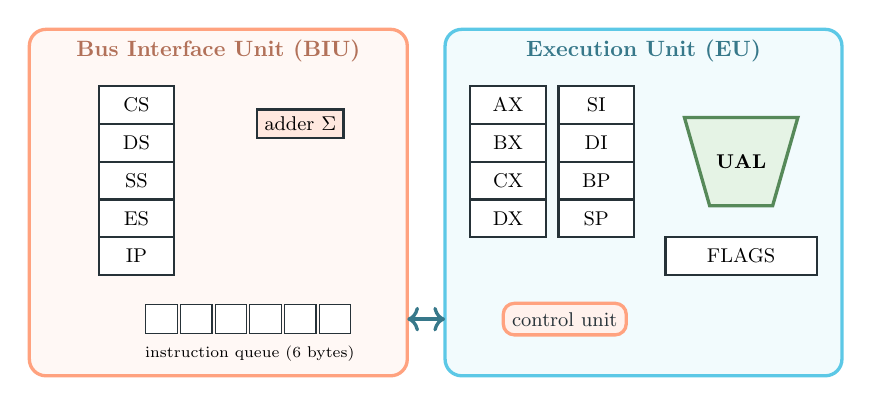
\begin{tikzpicture}[scale=0.8, transform shape, r/.style={reg, minimum width=1.2cm, font=\codefont\small}]
        \draw[brandTeal, very thick, rounded corners=6pt, fill=brandTeal!8] (0.3,-3) rectangle (6.6,2.5);
        \node[font=\bfseries, text=tealDeep] at (3.45,2.15) {Execution Unit (EU)};
        \foreach \n/\y in {AX/1.3, BX/0.7, CX/0.1, DX/-0.5} \node[r] at (1.3,\y) {\n};
        \foreach \n/\y in {SI/1.3, DI/0.7, BP/0.1, SP/-0.5} \node[r] at (2.7,\y) {\n};
        \draw[brandGreen!70!black, very thick, fill=brandGreen!20] (4.1,1.1) -- (5.9,1.1) -- (5.5,-0.3) -- (4.5,-0.3) -- cycle;
        \node[font=\bfseries\small] at (5,0.4) {UAL};
        \node[r, minimum width=2.4cm, font=\small] at (5,-1.1) {FLAGS};
        \node[unit=brandOrange, font=\small] at (2.2,-2.1) {control unit};
        \draw[brandOrange, very thick, rounded corners=6pt, fill=brandOrange!8] (-6.3,-3) rectangle (-0.3,2.5);
        \node[font=\bfseries, text=orangeDeep] at (-3.3,2.15) {Bus Interface Unit (BIU)};
        \foreach \n/\y in {CS/1.3, DS/0.7, SS/0.1, ES/-0.5, IP/-1.1} \node[r] at (-4.6,\y) {\n};
        \node[draw=brandDark, fill=brandOrange!25, thick, font=\small] at (-2,1) {adder $\Sigma$};
        \foreach \i in {0,...,5} \node[draw=brandDark, fill=white, minimum width=0.5cm, minimum height=0.45cm] at (-4.2+0.55*\i,-2.1) {};
        \node[font=\scriptsize] at (-2.8,-2.65) {instruction queue (6 bytes)};
        \draw[sahmT, <->] (-0.3,-2.1) -- (0.3,-2.1);
    \end{tikzpicture}
    \end{center}
    BIU: talks with memory and fetches in advance. EU: decodes and runs.
\end{frame}

\begin{frame}{The general registers}
    \begin{center}
    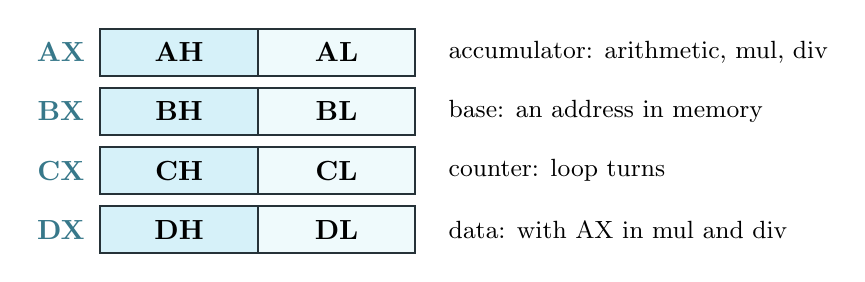
\begin{tikzpicture}[h/.style={draw=brandDark, thick, minimum width=2cm, minimum height=0.6cm, font=\codefont\bfseries}]
        \foreach \r/\n/\d [count=\i from 0] in {A/AX/{accumulator: arithmetic, mul, div},
                                             B/BX/{base: an address in memory},
                                             C/CX/{counter: loop turns},
                                             D/DX/{data: with AX in mul and div}} {
            \node[font=\codefont\bfseries, text=tealDeep] at (-1.5,-0.75*\i) {\n};
            \node[h, fill=brandTeal!25] at (0,-0.75*\i) {\r H};
            \node[h, fill=brandTeal!10] at (2,-0.75*\i) {\r L};
            \node[font=\small, anchor=west] at (3.3,-0.75*\i) {\d};
        }
    \end{tikzpicture}
    \end{center}
    If AX = \hex{1234}: AH = \hex{12}, AL = \hex{34}.
\end{frame}

\begin{frame}{Pointers, segments, IP and FLAGS}
    \begin{columns}[T]
        \column{0.48\textwidth}
        \small
        \begin{tabular}{|c|l|}
            \hline \ras{Reg.} & \ras{Job} \\ \hline
            SI, DI & source / destination index \\ \hline
            SP & top of the stack \\ \hline
            BP & data inside the stack \\ \hline
            IP & next instruction \\ \hline
        \end{tabular}
        \column{0.48\textwidth}
        \small
        \begin{tabular}{|c|l|}
            \hline \ras{Segment} & \ras{Start of\dots} \\ \hline
            CS & the code \\ \hline
            DS & the data \\ \hline
            SS & the stack \\ \hline
            ES & an extra segment \\ \hline
        \end{tabular}
    \end{columns}
    \vspace{6pt}
    \begin{center}
    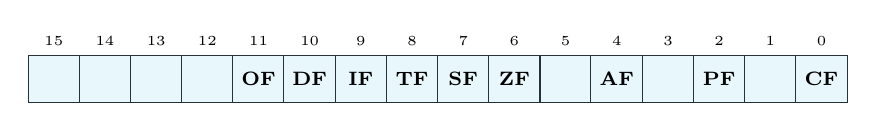
\begin{tikzpicture}[b/.style={draw=brandDark, minimum width=0.65cm, minimum height=0.6cm, font=\codefont\scriptsize\bfseries}]
        \foreach \n [count=\i from 0] in {{}, {}, {}, {}, OF, DF, IF, TF, SF, ZF, {}, AF, {}, PF, {}, CF} {
            \pgfmathtruncatemacro\bit{15-\i}
            \node[b, fill=brandTeal!15] at (0.65*\i, 0) {\n};
            \node[font=\codefont\tiny] at (0.65*\i, 0.48) {\bit};
        }
    \end{tikzpicture}
    \end{center}
\end{frame}

\begin{frame}{Segmented addressing}
    \begin{itemize}
        \item Registers are 16 bits (64 KB), but the address bus is 20 bits (1 MB).
        \item So an address uses \textbf{two} registers: \texttt{segment:offset}.
    \end{itemize}
    \begin{tbox}{\faLightbulb\quad The rule}
        \centering physical address $= \text{segment} \times 16 + \text{offset}$
    \end{tbox}
    \begin{pbox}{\faSmile\quad Analogy}
        Segment = street number, offset = house number in the street.
    \end{pbox}
\end{frame}

\begin{frame}{Example: CS = 1000H, IP = 0234H}
    \begin{columns}
        \column{0.5\textwidth}
        \begin{gbox}{\faShoePrints\quad Step by step}
            \begin{enumerate}
                \item $\hex{1000} \times 16 = \hex{10000}$.
                \item $\hex{10000} + \hex{0234} = \hex{10234}$.
            \end{enumerate}
        \end{gbox}
        1023:0004 gives the same address!
        \column{0.45\textwidth}
        \begin{center}
        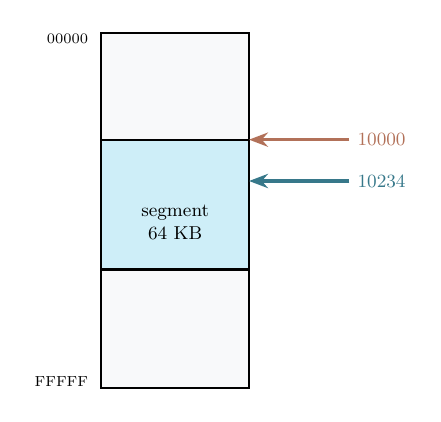
\begin{tikzpicture}[scale=0.75, transform shape]
            \draw[thick, fill=brandLight] (0,0) rectangle (2.5,-6);
            \node[font=\codefont\scriptsize, anchor=east] at (-0.1,-0.1) {00000};
            \node[font=\codefont\scriptsize, anchor=east] at (-0.1,-5.9) {FFFFF};
            \fill[brandTeal!30] (0,-1.8) rectangle (2.5,-4);
            \draw[thick] (0,-1.8) rectangle (2.5,-4);
            \node[font=\small, align=center] at (1.25,-3.2) {segment\\64 KB};
            \draw[sahmO] (4.2,-1.8) node[right, font=\small] {10000} -- (2.5,-1.8);
            \draw[sahmT] (4.2,-2.5) node[right, font=\small] {10234} -- (2.5,-2.5);
        \end{tikzpicture}
        \end{center}
    \end{columns}
\end{frame}

\begin{frame}{Default pairs and addressing modes}
    \begin{columns}[T]
        \column{0.4\textwidth}
        \small
        \begin{tabular}{|c|c|}
            \hline \ras{Offset} & \ras{Segment} \\ \hline
            IP & CS \\ \hline
            SP, BP & SS \\ \hline
            BX, SI, direct & DS \\ \hline
            DI (strings) & ES \\ \hline
        \end{tabular}
        \column{0.56\textwidth}
        \small
        \begin{tabular}{|l|l|}
            \hline \ras{Mode} & \ras{EA} \\ \hline
            \code{[0200h]} & \hex{0200} \\ \hline
            \code{[bx]} & BX \\ \hline
            \code{[bx+4]} & BX + 4 \\ \hline
            \code{[bx+si+4]} & BX + SI + 4 \\ \hline
        \end{tabular}
    \end{columns}
    \vspace{6pt}
    \begin{gbox}{\faShoePrints\quad \code{[bx+si+4]} with DS = 2000, BX = 0100, SI = 0020}
        EA $= \hex{0124}$, physical address $= \hex{20000} + \hex{0124} = \hex{20124}$.
    \end{gbox}
\end{frame}

\begin{frame}{A first program}
    \asm{ch3/hello.asm}
    \screen{ch3/hello.out}
    In a .COM program, CS = DS = SS = ES, and the code starts at \hex{100} (\code{org 100h}).
\end{frame}

\begin{frame}{The program in memory}
    \begin{center}
    \begin{tabular}{|c|l|l|}
        \hline \ras{Offset} & \ras{Bytes} & \ras{Content} \\ \hline
        0100 & {\codefont 8D 16 09 01} & \code{lea dx, msg} \\ \hline
        0104 & {\codefont B4 09} & \code{mov ah, 09h} \\ \hline
        0106 & {\codefont CD 21} & \code{int 21h} \\ \hline
        0108 & {\codefont C3} & \code{ret} \\ \hline
        0109 & {\codefont 53 61 6C 61 6D \dots} & ``Salam\dots'' \\ \hline
    \end{tabular}
    \end{center}
    \begin{obox}{\faExclamationTriangle\quad Watch out}
        Data goes \textbf{after} \code{ret}; otherwise the processor runs the letters as instructions.
    \end{obox}
\end{frame}

\begin{frame}{How \code{mov cx, [si]} runs}
    \begin{center}
    \small
    \begin{tabularx}{0.95\linewidth}{|c|c|L|}
        \hline \ras{Step} & \ras{Unit} & \ras{What happens} \\ \hline
        1 & BIU & fetches the bytes 8B 0C into the queue \\ \hline
        2 & EU & decodes: ``word from memory to CX, address in SI'' \\ \hline
        3 & EU & EA = SI = \hex{0112} \\ \hline
        4--5 & BIU & sends $\text{DS} \times 16 + \hex{0112}$, gets \hex{ABCD} \\ \hline
        6 & EU & CX = \hex{ABCD}; the flags do not change \\ \hline
    \end{tabularx}
    \end{center}
\end{frame}

\begin{frame}{Transfer: \code{mov}, \code{xchg}, \code{lea}}
    \begin{columns}[T]
        \column{0.6\textwidth}
        \asm{ch3/transfer.asm}
        \column{0.37\textwidth}
        \small
        \begin{tabular}{|c|c|c|}
            \hline \ras{Line} & \ras{AX} & \ras{BX} \\ \hline
            4 & 1234 & 0000 \\ \hline
            6 & 1234 & 3412 \\ \hline
            7 & 3412 & 1234 \\ \hline
        \end{tabular}
        \vspace{4pt}
        Line 8: SI = 0112 (address).\\
        Line 9: CX = ABCD (content).
    \end{columns}
\end{frame}

\begin{frame}{Arithmetic}
    \begin{columns}[T]
        \column{0.55\textwidth}
        \asm{ch3/arith.asm}
        \column{0.42\textwidth}
        \small
        AL: 25, 42, 40, 41, 40, then \textbf{\hex{D8}} $= -40$.
        \begin{gbox}{\faShoePrints\quad $-40$}
            $0010\,1000 \rightarrow 1101\,0111 \rightarrow +1 = \hex{D8}$
        \end{gbox}
    \end{columns}
\end{frame}

\begin{frame}{Multiply and divide}
    \begin{center}
    \small
    \begin{tabular}{|c|c|c|}
        \hline \ras{Instruction} & \ras{Operation} & \ras{Result} \\ \hline
        \code{mul bl} & AL $\times$ BL & AX \\ \hline
        \code{mul cx} & AX $\times$ CX & DX:AX \\ \hline
        \code{div bl} & AX $\div$ BL & AL = quotient, AH = remainder \\ \hline
    \end{tabular}
    \end{center}
    Real results: $12 \times 11$ gives AX = \hex{0084}; $300 \times 500$ gives DX:AX = 0002:49F0 (150000);
    $47 \div 5$ gives AX = \hex{0209} (quotient 9, remainder 2).
\end{frame}

\begin{frame}{Adding 32-bit numbers: \code{adc}}
    \asm{ch3/add32.asm}
    The carry of the low words (CF = 1) is added by \code{adc}: DX:AX = 0002:0000.
\end{frame}

\begin{frame}{Logic and shifts}
    \begin{columns}[T]
        \column{0.62\textwidth}
        \asm{ch3/logic.asm}
        \column{0.35\textwidth}
        \small
        \begin{itemize}
            \item \code{and}: switch bits off
            \item \code{or}: switch bits on
            \item \code{xor}: flip bits
            \item \code{shl}/\code{shr}: $\times 2$ / $\div 2$
        \end{itemize}
        BL: 5, 10, 20, 10.
    \end{columns}
\end{frame}

\begin{frame}{Jumps}
    \begin{center}
    \small
    \begin{tabular}{|l|l|}
        \hline \ras{Instruction} & \ras{Jumps if\dots} \\ \hline
        \code{jmp} & always \\ \hline
        \code{je}, \code{jne} & equal, not equal (ZF) \\ \hline
        \code{jg}, \code{jl} & greater, less (\textbf{signed}) \\ \hline
        \code{ja}, \code{jb} & above, below (\textbf{unsigned}) \\ \hline
    \end{tabular}
    \end{center}
    \code{cmp a, b} computes $a - b$ and sets the flags; the jump reads them.
    For the same bits \hex{C8}: \code{ja} sees 200 > 100, but \code{jg} sees $-56 < 100$.
\end{frame}

\begin{frame}{If \dots\ else}
    \begin{columns}[T]
        \column{0.58\textwidth}
        \asms{ch3/ifelse.asm}
        \column{0.39\textwidth}
        \screen{ch3/ifelse.out}
        \small
        \begin{itemize}
            \item Line 5: $7 - 12 < 0$.
            \item Line 6: no jump.
            \item Line 8: \code{jmp show} is needed, or we also run line 10.
        \end{itemize}
    \end{columns}
\end{frame}

\begin{frame}{Loops with \code{loop}}
    \begin{columns}[T]
        \column{0.55\textwidth}
        \asm{ch3/loopsum.asm}
        \column{0.42\textwidth}
        \small
        \code{loop} = \code{dec cx}, then jump if CX $\neq 0$.
        \begin{center}
        \begin{tabular}{|c|c|}
            \hline \ras{CX} & \ras{AX after add} \\ \hline
            10 & 10 \\ \hline 9 & 19 \\ \hline 8 & 27 \\ \hline \dots & \dots \\ \hline 1 & \textbf{55} \\ \hline
        \end{tabular}
        \end{center}
    \end{columns}
\end{frame}

\begin{frame}{Machine code}
    \begin{columns}[T]
        \column{0.42\textwidth}
        \small
        \begin{tabular}{|l|l|}
            \hline \ras{Bytes} & \ras{Instruction} \\ \hline
            {\codefont B8 34 12} & \code{mov ax, 1234h} \\ \hline
            {\codefont 89 C3} & \code{mov bx, ax} \\ \hline
            {\codefont 04 05} & \code{add al, 5} \\ \hline
            {\codefont 88 07} & \code{mov [bx], al} \\ \hline
            {\codefont EB 01} & \code{jmp fin} \\ \hline
        \end{tabular}
        \column{0.55\textwidth}
        \begin{gbox}{\faShoePrints\quad 89 C3}
            \small 89 = 100010\,0\,1: \code{mov}, d = 0, w = 1 (16 bits).\\
            C3 = 11\,000\,011: mod = register, reg = AX, r/m = BX.
        \end{gbox}
        \small EB 01: jump 1 byte forward (relative).
    \end{columns}
\end{frame}

\begin{frame}{Input and output with DOS}
    \begin{columns}[T]
        \column{0.45\textwidth}
        \small
        \begin{tabular}{|c|l|}
            \hline \ras{AH} & \ras{\code{int 21h}} \\ \hline
            01 & read a key into AL \\ \hline
            02 & print DL \\ \hline
            09 & print a \$ string (DX) \\ \hline
            4C & end the program \\ \hline
        \end{tabular}
        \vspace{6pt}
        Ports: \code{in al, 60h}, \code{out 61h, al}.
        \column{0.52\textwidth}
        \asm[firstline=7, firstnumber=7, lastline=17]{ch3/io.asm}
        \screen{ch3/io.out}
    \end{columns}
\end{frame}

\begin{frame}{The stack}
    \begin{itemize}
        \item LIFO: \textbf{last in, first out}, like a pile of plates.
        \item \code{push}: \nql{SP}{SP - 2}, then write. \quad \code{pop}: read, then \nql{SP}{SP + 2}.
    \end{itemize}
    \begin{center}
    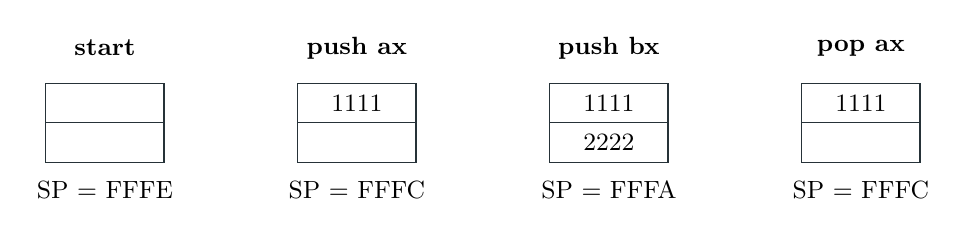
\begin{tikzpicture}[c/.style={draw=brandDark, fill=white, minimum width=1.5cm, minimum height=0.5cm, font=\codefont\small}]
        \foreach \t/\x/\v/\w/\sp in {{start}/0/{}/{}/FFFE, {push ax}/3.2/1111/{}/FFFC,
                                    {push bx}/6.4/1111/2222/FFFA, {pop ax}/9.6/1111/{}/FFFC} {
            \node[font=\small\bfseries] at (\x,1) {\t};
            \node[c] at (\x,0.3) {\v}; \node[c] at (\x,-0.2) {\w};
            \node[font=\codefont\small] at (\x,-0.8) {SP = \sp};
        }
    \end{tikzpicture}
    \end{center}
    After \code{pop ax} and \code{pop bx}, AX and BX have swapped (real run).
\end{frame}

\begin{frame}{Procedures: \code{call} and \code{ret}}
    \begin{columns}[T]
        \column{0.58\textwidth}
        \asms[firstline=10, firstnumber=10, lastline=29]{ch3/procnum.asm}
        \column{0.39\textwidth}
        \small
        \begin{itemize}
            \item \code{call} pushes the return address.
            \item \code{ret} pops it into IP.
            \item The stack reverses the digits 6, 2, 0, 2.
        \end{itemize}
        \screen{ch3/procnum.out}
    \end{columns}
\end{frame}

\begin{frame}{Parameters on the stack}
    \begin{columns}[T]
        \column{0.5\textwidth}
        \asm[firstline=12, firstnumber=12, lastline=19]{ch3/procstack.asm}
        \small \code{ret 4} also removes the two parameters.
        \column{0.47\textwidth}
        \begin{center}
        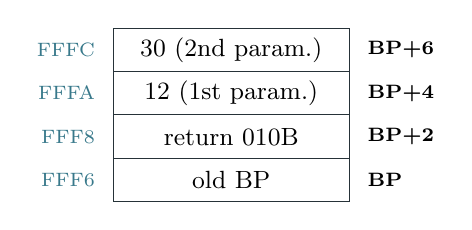
\begin{tikzpicture}[c/.style={draw=brandDark, fill=white, minimum width=3cm, minimum height=0.55cm, font=\small}]
            \foreach \ad/\v/\l [count=\i from 0] in {FFFC/{30 (2nd param.)}/{BP+6}, FFFA/{12 (1st param.)}/{BP+4},
                                                   FFF8/{return 010B}/{BP+2}, FFF6/{old BP}/{BP}} {
                \node[c] (n\i) at (0,-0.55*\i) {\v};
                \node[font=\codefont\scriptsize, text=tealDeep, left=0.1cm of n\i] {\ad};
                \node[font=\codefont\scriptsize\bfseries, right=0.1cm of n\i] {\l};
            }
        \end{tikzpicture}
        \end{center}
        \small $12 + 30 = 42$ in AX.
    \end{columns}
\end{frame}

\begin{frame}{Interrupts}
    \begin{columns}[T]
        \column{0.5\textwidth}
        \small
        \begin{itemize}
            \item Kinds: hardware, software, exceptions.
            \item The address of handler $n$ is at $4n$.
            \item \code{int n} saves FLAGS, CS, IP; \code{iret} comes back.
        \end{itemize}
        \column{0.47\textwidth}
        \asms[firstline=4, firstnumber=4, lastline=19]{ch3/myint.asm}
        \screen{ch3/myint.out}
    \end{columns}
\end{frame}

\begin{frame}{Summary}
    \begin{tbox}{\faCheckCircle\quad Remember}
        \begin{itemize}
            \item physical address $= \text{segment} \times 16 + \text{offset}$.
            \item \code{cmp} sets the flags; jumps read them (signed: \code{jg}, unsigned: \code{ja}).
            \item The stack (LIFO) keeps return addresses, registers and parameters.
        \end{itemize}
    \end{tbox}
\end{frame}

\end{document}
